\chapter{Results, Validation and Discussion}
\label{ch:results}

\section{Physical-Layer Preamble Capture (Finding 1)}
\label{sec:r1capture}

Using the srsRAN 5G physical-layer implementation~\cite{srsran} under 3GPP TR~38.901 channel models,
we evaluated the relative relay power advantage required to capture the candidate gNB's PRACH correlator.
The simulation executed 2000 Monte Carlo trials per configuration at 30\,kHz ($\mu=1$) with preamble
format~B4.

\begin{table}[htbp]
  \centering
  \caption{Relay received power advantage relative to direct UE path required to capture the candidate cell
  correlator (2000 trials per point), shown for three representative delays spanning the full swept range
  7--32 units; the threshold is delay-invariant, as the near-identical rows below confirm.}
  \label{tab:capture}
  \small
  \begin{tabular}{@{}c rrrr@{}}
    \toprule
    Relay Delay $\Delta$ & \multicolumn{2}{c}{Flat Rayleigh Fading} & \multicolumn{2}{c}{20-Tap Urban Multipath} \\
    \cmidrule(lr){2-3} \cmidrule(lr){4-5}
    ($T_{\mathrm{unit}}$) & 50\% Capture & 90\% Capture & 50\% Capture & 90\% Capture \\
    \midrule
    7  & $+0.23$\,dB & $+9.89$\,dB & $+0.05$\,dB & $+5.53$\,dB \\
    16 & $+0.21$\,dB & $+9.87$\,dB & $+0.09$\,dB & $+5.31$\,dB \\
    32 & $+0.22$\,dB & $+9.88$\,dB & $+0.06$\,dB & $+5.32$\,dB \\
    \bottomrule
  \end{tabular}
\end{table}

\begin{figure}[htbp]
  \centering
  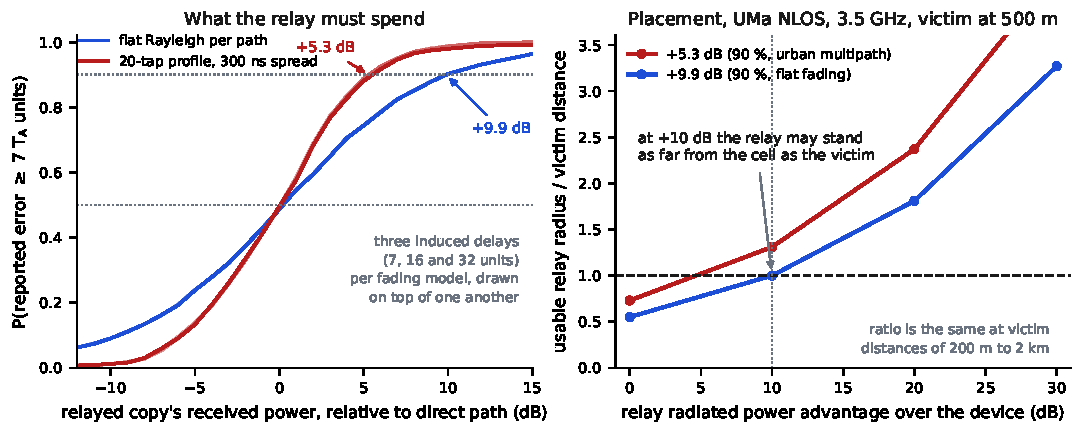
\includegraphics[width=\textwidth]{figures/atk05a_capture.pdf}
  \caption{Left: Preamble capture probability versus relay power advantage. Right: Admissible relay
  operating radius normalized by victim distance under TR~38.901 path loss.}
  \label{fig:capture}
\end{figure}

As shown in \cref{tab:capture} and \cref{fig:capture}, three critical properties emerge:
\begin{enumerate}\itemsep1pt
  \item \textbf{Delay-Invariant Power Threshold:} The 90\% capture threshold remains constant at $+9.9$\,dB
        under flat fading across all injected delays (7 to 32 units). The PRACH correlation sequence has
        a flat frequency spectrum; thus, the correlator contest is decided strictly by relative received
        amplitude rather than temporal displacement.
  \item \textbf{Multipath Reduces Attacker Cost:} Under realistic 20-tap urban multipath (300\,ns delay
        spread), the required 90\% power advantage drops by 4.6\,dB to $+5.3$\,dB. Multipath disperses
        preamble energy into reflection clusters, increasing the probability that a relayed multipath tap
        produces the dominant correlation peak.
  \item \textbf{Geographic Feasibility:} Under TR~38.901 urban path loss, a $+10$\,dB power advantage
        permits the relay to operate anywhere within a radius $r \le d$ from the candidate cell,
        confirming that the attacker faces no delicate spatial positioning constraints.
\end{enumerate}

\section{Decodability Boundary and Receiver Retracking}
\label{sec:r1boundary}

To determine the exact point where timing misalignment destroys uplink reception, we evaluated the
OpenAirInterface (OAI)~\cite{oai} LDPC coding chain under time-domain timing offsets. Link failure is
defined as coded $\text{BLER} \ge 0.99$.

While the theoretical cyclic prefix guard interval spans 9 units (\cref{eq:cp9}), channel delay spread
and receiver filtering consume part of this budget in practice. The empirical decodability boundary in
the early transmission direction spans \textbf{6 to 8 units (median 7 units)}, corresponding to
$1.82\,\mu\text{s}$ at 30\,kHz. Beyond 12 units, post-equalization SNR drops below $-24$\,dB across all
modulation orders (QPSK through 256-QAM) and code rates (0.19 to 0.66).

\begin{figure}[htbp]
  \centering
  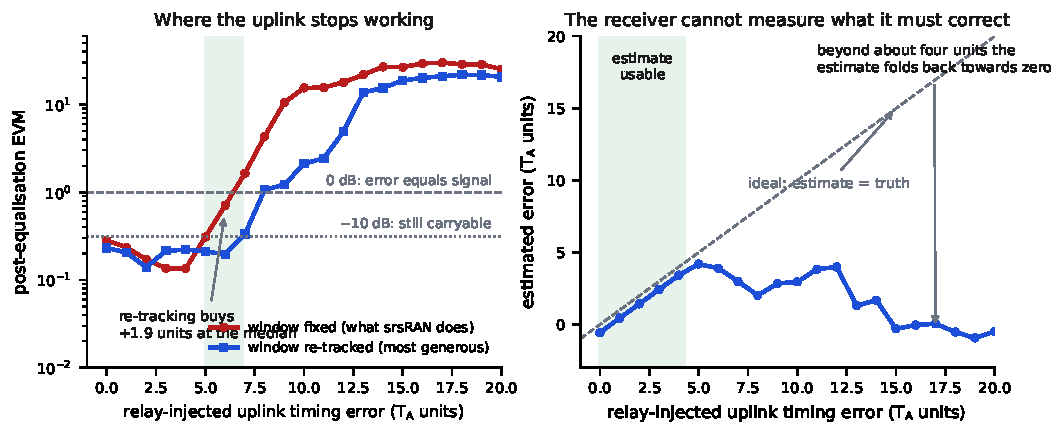
\includegraphics[width=\textwidth]{figures/atk05b_retrack.pdf}
  \caption{Left: Post-equalization EVM versus timing error before and after receiver tracking. Right:
  Receiver timing estimation error, exhibiting foldback towards zero beyond 4 units.}
  \label{fig:retrack}
\end{figure}

\paragraph{Failure of Receiver Re-tracking:} Modern 5G base stations employ digital tracking loops to track
sub-microsecond timing drift from mobile UEs. We evaluated whether this tracking mechanism could detect
a 7-unit error and shift its receiver FFT window to rescue the connection. As shown in \cref{fig:retrack},
closed-loop tracking provides a maximum correction of only $+4.38$ units (median $+1.86$), beyond which
phase ambiguity causes the estimator to fold back toward zero rather than continue tracking the true
error. At 7 units of true error, the receiver tracking loop is ineffective and cannot detect or correct
the error.

\section[Window Confinement Mitigation (ZCZ)]{Window Confinement Mitigation via ZCZ Search Window}
\label{sec:r1zcz}

The gNB PRACH search window is governed by \texttt{zeroCorrelationZoneConfig} (ZCZ), which sets the
cyclic shift $N_{\mathrm{CS}}$. A correlator cannot report delays exceeding its search window.

\begin{table}[htbp]
  \centering
  \caption{PRACH search window and damaging error probability by ZCZ configuration (2000 trials).}
  \label{tab:zcz}
  \small
  \begin{tabular}{@{}c r rrr@{}}
    \toprule
    ZCZ & Window & \multicolumn{3}{c}{$P(\text{Damaging Error})$} \\
    \cmidrule(lr){3-5}
    Index & ($T_{\mathrm{unit}}$) & $0$\,dB & $+3$\,dB & $+6$\,dB \\
    \midrule
    \multicolumn{5}{@{}l}{\emph{Safe Configurations (Search Window $< 7\,T_{\mathrm{unit}}$)}} \\
    1  & 0.40  & 0.000 & 0.000 & 0.000 \\
    2  & 2.00  & 0.000 & 0.000 & 0.000 \\
    3  & 3.60  & 0.000 & 0.000 & 0.000 \\
    4  & 4.80  & 0.000 & 0.000 & 0.000 \\
    5  & 6.40  & 0.000 & 0.000 & 0.000 \\
    \midrule
    \multicolumn{5}{@{}l}{\emph{Exposed Configurations (Search Window $\ge 7\,T_{\mathrm{unit}}$)}} \\
    8  & 10.00 & 0.886 & 0.931 & 0.967 \\
    9  & 11.60 & 0.986 & 0.994 & 0.996 \\
    10 & 13.20 & 1.000 & 1.000 & 1.000 \\
    12 & 18.80 & 0.718 & 0.836 & 0.909 \\
    15 & 46.40 & 0.487 & 0.650 & 0.786 \\
    \bottomrule
  \end{tabular}
\end{table}

As shown in \cref{tab:zcz}, configurations 1 through 5 constrain the searchable delay below the 7-unit
decodability boundary, completely eliminating damaging errors ($P=0$). However, this protection trades
directly against cell radius: ZCZ configurations $\le 5$ limit maximum cell radius to under 500\,m,
making them unusable in macro-cell deployments.

\section{Scheduling Request Failure Under Corrupted Timing Advance}
\label{sec:r2sr}

Next, we evaluate the decodability of PUCCH Format~0 Scheduling Requests under timing errors. We evaluated
srsRAN's physical-layer Format~0 detector across 2000 trials per point.

\begin{figure}[htbp]
  \centering
  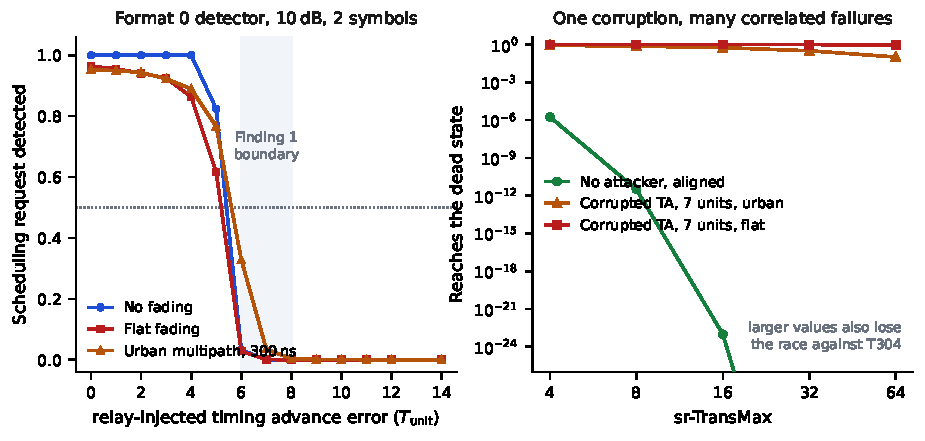
\includegraphics[width=\textwidth]{figures/atk16_sr.pdf}
  \caption{Left: PUCCH Format~0 SR recovery probability versus \TA{} error across channel models.
  Right: Deterministic escalation to counter exhaustion ($P > 0.99$) under 7 units of \TA{} error.}
  \label{fig:sr}
\end{figure}

\paragraph{Analytical Coherence Collapse:} PUCCH Format~0 transmits a single bit via a cyclic shift of a
base sequence across the 12 subcarriers of one resource block. An uncompensated timing offset introduces
an escalating phase rotation across the subcarriers ($e^{-j 2\pi k \Delta f \tau}$), causing destructive
phase cancellation during coherent receiver correlation. Consequently, the correlation peak drops below
the gNB's detection threshold ($0.5273$ in srsRAN) by 6 to 7 units of error, as confirmed by our
simulations in \cref{tab:srports}.

\begin{table}[htbp]
  \centering
  \caption{PUCCH Format~0 SR detection probability versus receive antenna ports and timing error
  (Flat Rayleigh fading, 10\,dB SNR, 2000 trials).}
  \label{tab:srports}
  \small
  \begin{tabular}{@{}l rrrrrr@{}}
    \toprule
    Receive Ports & Threshold & 0 units & 5 units & 6 units & 7 units & 8 units \\
    \midrule
    1 Port  & 0.5273 & 0.964 & 0.616 & 0.028 & 0.0005 & \textbf{0.000} \\
    2 Ports & 0.3455 & 0.998 & 0.968 & 0.432 & 0.0010 & \textbf{0.000} \\
    4 Ports & 0.2545 & 1.000 & 1.000 & 0.955 & 0.0205 & \textbf{0.000} \\
    \bottomrule
  \end{tabular}
\end{table}

\paragraph{Simulation Verification:} As shown in \cref{fig:sr} and \cref{tab:srports}, SR detection
collapses abruptly between 5 and 7 units. At 7 units of error, SR recovery probability is $0.0005$ at
1 port and $0.0205$ at 4 ports. At 8 units of error, not a single SR is detected in 2000 trials across
any antenna configuration. Because the failure is caused by phase decorrelation rather than noise,
increasing SNR from $-3$\,dB to $+20$\,dB yields 0\% recovery. The target gNB is blind to the request.

\section{Parameter Space Sweep and Outage Evaluation}
\label{sec:r2}

We evaluated the complete 5400-configuration space defined in \cref{sec:m2model} across varying handover
supervision windows (\texttt{t304}).

\begin{figure}[htbp]
  \centering
  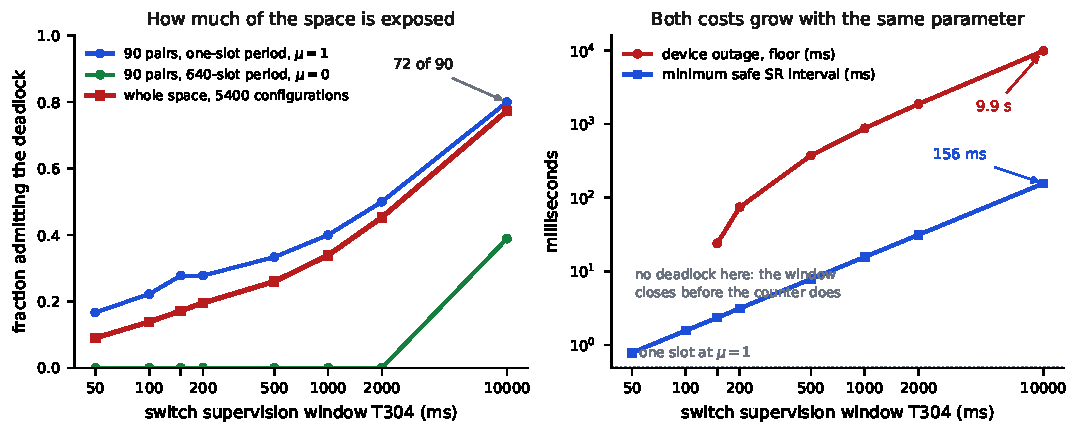
\includegraphics[width=\textwidth]{figures/atk16_space.pdf}
  \caption{Left: Percentage of configurations reaching deadlock versus \texttt{t304} duration. Right:
  Deadlock outage duration $T_{\text{dead}}$ trade-off.}
  \label{fig:space}
\end{figure}

As shown in \cref{fig:space}, deadlock is reached in 9.0\% of configurations at $\texttt{t304}=50$\,ms,
increasing to 27.8\% at 200\,ms, and reaching 77.4\% at 10\,s. In terrestrial deployments where
$\texttt{t304}=200$\,ms is standard, counter exhaustion induces an average dead interval of
$T_{\text{dead}} \approx 72$\,ms. With longer switch windows, $T_{\text{dead}}$ exceeds several seconds.

\section{The Safe Configuration Rule}
\label{sec:rule}

From \cref{eq:exhaust}, counter exhaustion occurs before T304 expiry whenever $T_{\text{exhaust}} < \texttt{t304}$.
Consequently, an operator can guarantee immunity from this deadlock if and only if:
\begin{equation}
  \texttt{sr-TransMax} \times T_{\text{interval}} \;\ge\; \texttt{t304}.
  \label{eq:rule}
\end{equation}
When \cref{eq:rule} is satisfied, T304 expires prior to counter exhaustion, safely invoking the standard
RRC connection re-establishment procedure.

\begin{table}[htbp]
  \centering
  \caption[Minimum safe SR interval satisfying Equation~(5.2)]{Minimum SR interval required to satisfy \cref{eq:rule} at $\texttt{sr-TransMax}=64$, and resulting latency penalty relative to 0.5\,ms baseline. The final row applies to Non-Terrestrial Network (NTN) supervision windows; terrestrial deployments use $\texttt{t304} \le 1$\,s.}
  \label{tab:rule}
  \small
  \begin{tabularx}{\textwidth}{@{}X c c r@{}}
    \toprule
    \texttt{t304} Duration & Minimum Safe SR Interval & Minimum \texttt{sr-ProhibitTimer} & Latency Penalty \\
    \midrule
    100\,ms   & 1.56\,ms   & \texttt{ms2}   & $3.1\times$ \\
    200\,ms   & 3.13\,ms   & \texttt{ms4}   & $6.2\times$ \\
    1000\,ms  & 15.63\,ms  & \texttt{ms16}  & $31.2\times$ \\
    10\,s (NTN) & 156.25\,ms & \texttt{ms192} & $312.5\times$ \\
    \bottomrule
  \end{tabularx}
\end{table}

However, enforcing \cref{eq:rule} imposes a severe performance trade-off (\cref{tab:rule}): at
$\texttt{t304}=200$\,ms, ensuring safety requires stretching the SR interval by $6.2\times$, degrading
application latency. Furthermore, 3GPP Release~19 dynamically selects the SR configuration via a 3-bit index in the
unauthenticated LTM Cell Switch Command MAC CE, bypassing static deployment audits.

\section{Independent Deployment Verification (Amarisoft)}
\label{sec:deployed}

We verified the parameters of both findings against a published commercial LTM setup from
Amarisoft~\cite{amarisoft2026ltm} (\cref{tab:deployed}).

\begin{table}[htbp]
  \centering
  \caption{Audit of published Amarisoft commercial LTM configuration~\cite{amarisoft2026ltm}.}
  \label{tab:deployed}
  \small
  \begin{tabularx}{\textwidth}{@{}p{5.0cm} p{3.2cm} X@{}}
    \toprule
    Configuration Parameter & Commercial Value & Security Verdict \& Finding \\
    \midrule
    \texttt{zero\-Correlation\-Zone\-Config} & 15 (Window: 46.4 units) & \textbf{Vulnerable to Finding~1} ($P(\text{capture})=0.78$) \\
    \texttt{sr-TransMax} & \texttt{n64} & Safe under default $\texttt{t304} = 1000$\,ms ($T_{\text{exhaust}} = 1280$\,ms) \\
    SR Periodicity / Prohibit & \texttt{sl40} (20\,ms) / absent & Governs escalation time ($T_{\text{exhaust}} = 1.28$\,s) \\
    \texttt{t304} Supervision Window & \texttt{ms1000} (1000\,ms) & \textbf{Vulnerable to Finding~2} if operator configures $\texttt{t304} \ge 2000$\,ms \\
    \bottomrule
  \end{tabularx}
\end{table}

The deployment chooses ZCZ~15, exposing a wide 46.4-unit search window that leaves Finding~1 completely
effective. For Finding~2, the vendor configured a conservative 20\,ms SR periodicity, rendering it
safe at $\texttt{t304}=1000$\,ms, but exposing it whenever $\texttt{t304}$ is set to 2\,s or higher.

\section{Inadequacy of Existing Defenses}
\label{sec:detect}

We evaluated four existing cellular defense mechanisms:
\begin{itemize}\itemsep2pt
  \item \textbf{Standardized 3GPP Counters (TS~28.552~\cite{3gpp28552}):} 3GPP performance management
        defines counters for handover execution, but contains no counter tracking intra-handover
        interruption duration. Deadlocked UEs simply appear as silent drops after T304 expiry.
  \item \textbf{Successful Handover Report (SHR, TS~38.300~\cite{3gpp38300}):} SHR records slow switches
        based on elapsed fractions of T304. However, it cannot distinguish between RF channel fading and
        corrupted \TA{}.
  \item \textbf{Dey and Patra's Handover Classifier~\cite{dey2025secure}:} This detector localizes
        adversaries using features observed during failure. In our attack, the relay acts during early
        acquisition and departs; by the time the switch executes, the attacker is absent, rendering
        real-time localization ineffective.
  \item \textbf{MAC CE Integrity Protection (TR~33.801-01~\cite{3gpp33801}):} Cryptographic signing of
        MAC CEs does not prevent the attack. The candidate \TA{} measurement itself is corrupted prior to
        encapsulation; thus, the gNB will compute a valid integrity tag over the already-corrupted \TA{}.
\end{itemize}
